\documentclass[10pt, twocolumn]{IEEEtran}
% Leaving this next line in to periodically check how many Normal People Pages were written
%\documentclass[12pt, letterpaper]{article}
\usepackage[utf8]{inputenc}
\usepackage{graphicx}
\usepackage[style=apa, backend=biber]{biblatex}
\addbibresource{paper.bib}

\title{Granular synthesis for instrument makers}
\author{	
	\IEEEauthorblockN{Daniël Kamp\\}
    \IEEEauthorblockA{HKU University of the Arts Utrecht
    \\daniel.kamp@student.hku.nl}
    }
\date{April 2022}

\begin{document}

\maketitle

\begin{abstract}
This writing sheds light onto various forms of granular synthesis. It analyses some existing implementations, explains the inner workings of such a system, and provides insight into human interfaces to use this method of sound generation.
\end{abstract}

\section*{Introduction}
Granular synthesis is a versatile form of sample-based (digital) sound synthesis. It uses short slices of recorded audio to create new, rich sounds. These slices can be layered, stretched, spread, and in other ways processed to create vast soundscapes with relative ease. \\
This writing aims to demystify the technical aspects of granular synthesis, and provide a comprehensive insight for instrument makers who want to make use of the technique.

\section{What is granular synthesis?}
This first part tells a brief history of granular synthesis, explains the components of a system implementing this technique, and lists some reference instruments.

\subsection{A brief history}
Granular synthesis as it's known today is a form of digital sound synthesis, which is based on the processing of small slices of sampled audio known as "grains". The underlying view on sound perception was first proposed by Hungarian-British physicist Dennis Gabor in an article titled \textit{Acoustical Quanta and the Theory of Hearing} (\cite{gabor47}). In this writing, Gabor theorized an approach to sound similar to concepts found in quantum mechanics.\\ Building on this theory, in the late 1950s, Greek composer Iannis Xenakis started experimenting with the technique, stitching together many tiny slices of tape to create new sounds (\cite{robindore96}). Inspired by Xenakis during a 1972 workshop taught by the former, composer Curtis Roads eventually created the first computer software implementing this synthesis paradigm in 1974 (\cite{opie03}). His code produced a 30-second long piece titled Klang-1, using three parameters: envelope, duration, and density. This software, however, did not operate in real-time, and producing this piece of music took multiple days. The first real-time implementation of the principle came from Canadian composer Barry Truax, who developed GSX (1986) and GSAMX (1987) (\cite{truax88}). \\
Since then, granular synthesis has established itself as a pillar of modern digital sound generation. More approachable implementations of the technique, like Robert Henke's Granulator (2011), made it possible for anyone with a computer to explore its vast new possibilities in sound. Today, dozens of granular synthesizers are available, each offering a different approach to a 75-year-old concept.
%since then numerous implementations: robert henke popular granulator, hardware instruments, etc, etc

%\subsection{Terminology}
%Througout this writing, it's expected that the reader has a basic knowledge of the workings of digital audio, and is familiar with the concept of sampling. For concepts beyond these basic principles, refer to the following list for an explanation of their meaning.
%
%\subsubsection*{Grain}
%A small slice of sound, typically below X ms in length, used in a granular audio system.

\subsection{General system overview}
This section describes the general anatomy of a granular synthesizer, and gives a broad overview of the building blocks that make up such a system. 

\begin{figure}[ht!]
	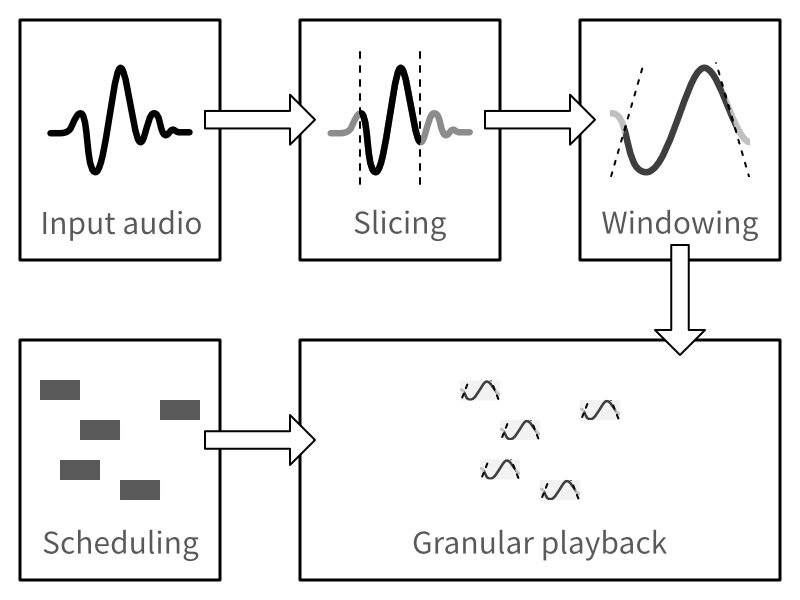
\includegraphics[width=\linewidth]{GranularDiagram.png}
	\caption{A simplified overview of a granular synthesis system.}
	\label{fig:block_diagram}
\end{figure}

\subsubsection{Sound source}
As its input, a granular system takes a sound stream. This stream can consist of sampled audio, live microphone input, or generated audio (such as sine waves). The content of this source material has an effect on the sounds one can generate: [insert comparison: transient-rich vs low-activity].

\subsubsection{Models}
There are four distinguishable models of granular synthesis: screen, cloud, stream, and spray (\cite{roads12}). The first of these, screen, was described by Xenakis and would run a series of time-frequency plots at a fixed time rate (\cite{xenakis63}). In layman's terms, this would be comparable to a flip book animation, used for sound instead. \\
The second model, clouds, generates a cloud of sound in which the individual grains are not bound to predefined parameters, but instead spread across specified ranges in a stochastic manner. This creates rich, unpredictable textures that are often used on a macro level within compositions. \\
The more regular counterpart of clouds is streams, in which grains are distributed in a deterministic process. In this model, the density (number of grains per second) determines a regular interval at which grains are played, creating a sort of rhythmic texture. This rhythm can be tweaked by modifying the grain density, through which one can create tone-like sounds. \\
A model that is used in modern digital granular synthesis is spray. This implementation makes it possible for users to draw the grains on a plot of frequency over time, which makes for an intuitive interaction model.

\subsubsection{Windowing and envelope}
Since the start position of grains is rather arbitrary, there is no telling what the amplitude of the first sample in the selection will be. Therefore, it's good practice, as it is in any digital audio application, to apply an envelope that trims off any rough edges that may exist in the source material. This envelope can be modified to a user's own insight through the parameters \textit{shape} and \textit{length}. \\
The shape of an envelope refers to its mathematical function. In this regard, there are four commonly used shapes: linear, square root, exponential, and Gaussian. The latter was proposed by Dennis Gabor in his original theory on granular sound, and is still commonly used. More recently, due to developments in the field of processing power in computers over the past 50-or-so years, it has become possible and commonplace to use other envelope shapes as well. Figure 2 [INSERT FIGURE 2] shows the four functions as a plot of amplitude over time.
Superseding their technical advantages, these envelopes have turned from makeshift solution to creative tool in the hands of resourceful artists. \\
The length of an envelope simply describes the time it takes for the signal to reach its full amplitude. By varying this number, one can change the character of the resulting sound. If a long \textit{attack} (rising edge of the envelope) is used, the resulting audio will sound more mellow compared to when a short attack time is applied.

\subsubsection{Duration and density}
Density, as mentioned previously, describes the number of grains played in one (1) second. Variations in this domain can roughly be split into two categories: \textit{deterministic} and \textit{stochastic}.\\
In a deterministic distribution, grains are played back with even spacing between them. This means that the resulting sound is of a regular nature.  \\

Stochastic distribution, on the other hand, adds a realm of uncertainty to the sound.

\subsection{Existing instruments}
This section lists a few instruments and effects that use granular synthesis. \\ Author's note: I selected open-source instruments of which the source code is freely available to the public. This way, I can give an in-depth comparison of the inner workings of these instruments. I'll use these and their concrete implementations as references throughout the rest of my research described in this writing.

\subsubsection{Mutable Instruments' Clouds}
Clouds is a Eurorack module developed and produced by Émilie Gillet (Mutable Instruments). Both the hardware files (schematics, CAD-files) and firmware source code are open-source and publicly available.\\
What?
- Eurorack module
- Open-source hardware and firmware
- Granular effect with built-in sound source\\
How?
- Clouds triggers one grain at a time
- Clouds uses a predetermined amount of grains (64 max)
- Clouds uses Look Up Tables for almost everything (filter, windowing, etc)

\subsubsection{Tasty Chips GR-1}
Here I describe GR-1.

\subsubsection{Argotlunar}
Argotlunar is a real-time granular VST and AudioUnit plugin created by Michael Ourednik. The source code of this software is open-source and available via GitHub.


\section{How does granular synthesis work?}
This part dives deeper into the inner workings of a granular system. Starting with a brief explanation of core audiological concepts that define how we experience sound on a short time scale, it then proceeds to explain concrete implementations of a granular synthesizer in C++. These examples are then compared through statistics about their performance, so a recommendation can be made based on system efficiency.

\subsection{Audiological concepts}
Here I SHORTLY describe the audiological concepts that make this system possible. AKA: why do we perceive lots of small ticks as a coherent sound, and IMPORTANT: what criteria does our system need to fit in order to be deemed a successful granular synthesizer. This makes our hypothesis concrete and closed off.
\subsection{Implementations}
In this section, implementations and methods are proposed for specific parts of the system. The next section will take execution metrics from these example implementations, and validate them by the requirements defined previously.
\subsubsection{Sound sourcing and selection}
This part lists different methods of sound sourcing and sample selection:
- Microphone or audio input
- Sample-based granular synthesis\\
For sample selection:
- Randomized selection
- Transient selection
\subsubsection{Trigger algorithms}
Here I write about different trigger algorithms: when does a grain get triggered, what conditions exist, and how can this be controlled in a musical manner?
\subsubsection{Windowing algorithms and approaches}
Here I write about different approaches to windowing: look-up tables, real-time calculation, pre-calculation, etc.
Note: Mutable Instruments uses LUTs, I want to use runtime calculation (insert tested efficiency of both)

\subsection{Efficiency}
This subsection looks at variables that impact system performance, and how manufacturers handle those. Note that these benchmarks were ran on a 2019 MacBook Pro ().

\section{How is granular synthesis used?}
This section looks at the human aspect of granular synthesis: what sounds does it produce, how is it controlled, and how can one play an instrument that uses this technique. KEEP THIS PART SHORT

\subsection{Human control}
This subsection looks at ways a human being can control a granular instrument. Common input methods like touch interfaces, sliders, knobs, and digital UIs are described and compared.

\subsection{Playability}
This subsection looks at how such instruments can be controlled in an artistic manner. It provides an insight into live performance methods and some useful macros (maybe).

\section*{Conclusions}
This section summarizes my findings from the research, and gives a careful recommendation on implementing such system based on these results.

\printbibliography
\textit{All graphics in this writing were created by the author, unless otherwise noted.}

\end{document}